\documentclass[12pt]{article}
%packages
\usepackage[top=1in, bottom=1in, left=.75in, right=.75in]{geometry}
\usepackage{amsmath, enumerate}
\usepackage{fancyhdr,tabularx}
\usepackage{graphicx, xcolor, setspace, array}
\usepackage{txfonts}
\usepackage{multicol,coordsys,pgfplots}
\usepackage[scaled=0.86]{helvet}
\usepackage{anyfontsize}
\usepackage{tikz,pgfplots,cancel}
\usetikzlibrary{calc,arrows.meta}
\usetikzlibrary{positioning, quotes}

% specials
\renewcommand{\emph}[1]{\textsf{\textbf{#1}}}
\def\ra{\rightarrow}
\pgfplotsset{compat = newest}
\newcommand{\blank}[1]{\rule{#1}{0.75pt}}
\pgfplotsset{my style/.append style={axis x line=middle, axis y line=
middle, xlabel={$x$}, ylabel={$y$}}}
\newcommand{\be}{\begin{enumerate}}
\newcommand{\ee}{\end{enumerate}}
\newcommand{\ans}[1][1in]{\rule{#1}{.5pt}}
\newcommand{\ul}[1]{\underline{#1}}
\let\ds\displaystyle
\def\continued{{\emph {Continued....}}}
\def\continuing{{\emph {Problem \arabic{probcount} continued....}}\par\vskip 4pt}

%page setup
\parindent 0pt
\parskip 4pt
\pagestyle{fancy}
\fancyfoot[C]{\emph{\thepage}}
\fancyfoot[R]{} %%%%%% <-- Version Info
\fancyhead[L]{\ifnum \value{page} > 1\relax\emph{Math F113X: Exam 2}\fi}
\fancyhead[R]{\ifnum \value{page} > 1\relax\emph{Spring 2026}\fi}
\headheight 15pt
\renewcommand{\headrulewidth}{0pt}
\renewcommand{\footrulewidth}{0pt}

%%%%%
% Document Begins
%%%%%
\begin{document}
%%%%
% Front Page
%%%%
{\emph{\fontsize{26}{28}\selectfont Spring 2026 \hfill
\hfill Math F113X}}

\begin{center}
{\emph{
{\fontsize{32}{36}\selectfont Exam 2}}
}
\end{center}

\vfill
\emph{\fontsize{18}{22}\selectfont Name:\underline{\hspace{2in}}\hspace{2cm} Instructor: \underline{\hspace{2in}}}\\


\vfill
{\fontsize{18}{22}\selectfont\emph{Rules:}}

\begin{itemize}
\item Partial credit will be awarded, but you must show your work.

\item You may have a $3 \text{in} \times 5 \text{in} $ notecard with writing on both sides.

\item Calculators are allowed. 

\item Turn off anything that might go beep during the exam.

\end{itemize}




Good luck!

\vfill
\def\emptybox{\hbox to 2em{\vrule height 16pt depth 8pt width 0pt\hfil}}
\def\tline{\noalign{\hrule}}
\centerline{\vbox{\offinterlineskip
{
\bf\sf\fontsize{18pt}{22pt}\selectfont
\hrule
\halign{
\vrule#&\strut\quad\hfil#\hfil\quad&\vrule#&\quad\hfil#\hfil\quad
&\vrule#&\quad\hfil#\hfil\quad&\vrule#\cr
height 3pt&\omit&&\omit&&\omit&\cr
&Problem&&Possible&&Score&\cr\tline
height 3pt&\omit&&\omit&&\omit&\cr
&1&&12&&\emptybox&\cr\tline
&2&&12&&\emptybox&\cr\tline
&3&&12&&\emptybox&\cr\tline
&4&&12&&\emptybox&\cr\tline
&5&&12&&\emptybox&\cr\tline
&6&&10&&\emptybox&\cr\tline
&7&&15&&\emptybox&\cr\tline
&8&&15&&\emptybox&\cr\tline
&Extra Credit&&(4)&&\emptybox&\cr\tline
&Total&&100&&\emptybox&\cr
}\hrule}}}

\newpage

\begin{enumerate}
%%%%%%%%%%%%%
%%% Kruskal's + Spanning Trees
%%%%%%%%%%%%%
\item (12 pts.~total)

\begin{enumerate}

\item  (6 pts.) Perform Kruskal's algorithm to find a minimum weight spanning tree for the following graph. Draw your tree,  connecting the vertices provided, and determine the total weight.

\ 

\ 

%%%%%%%%%
% again

%\setlength{\tabcolsep}{2pt} % remove extra padding
%\renewcommand{\arraystretch}{1.1}
\hspace*{-.5in}
\begin{tabular}{p{0.25\textwidth} p{0.35\textwidth} p{0.25\textwidth}}

% -------- LEFT: TABLE --------
\centering
\vspace{0pt}
\begin{tabular}{c|c|c}
edge & weight & used? \\
\hline
eg & 1 & \\ \hline
bd & 2 & \\ \hline
ad & 3 & \\ \hline
de & 4 & \\ \hline
ab & 5 & \\ \hline
dg & 5 & \\ \hline
ef & 6 & \\ \hline
bc & 7 & \\ \hline
be & 8 & \\ \hline
cf & 9 & \\ \hline
ae & 11 & \\
\end{tabular}

&

% -------- MIDDLE: GRAPH --------
\centering
\vspace{0pt}
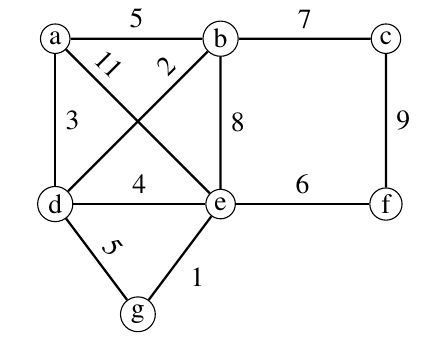
\begin{tikzpicture}[
    node style/.style={circle, draw, inner sep=1.5pt},
    every edge/.style={draw, thick},
    scale=0.7
]

% FIXED BOUNDING BOX (critical for alignment)
\path[use as bounding box] (-0.5,-2.2) rectangle (6.5,3.2);

\node[node style] (A) at (0, 3) {a};
\node[node style] (B) at (3, 3) {b};
\node[node style] (C) at (6, 3) {c};
\node[node style] (D) at (0, 0) {d};
\node[node style] (E) at (3, 0) {e};
\node[node style] (F) at (6, 0) {f};
\node[node style] (G) at (1.5, -2) {g};

\path (A) edge["5", above] (B);
\path (B) edge["7", above] (C);
\path (D) edge["4", above] (E);
\path (E) edge["6", above] (F);
\path (A) edge["3", left]  (D);
\path (B) edge["8", left]  (E);
\path (C) edge["9", left]  (F);
\path (B) edge["2",  sloped, pos=.2] (D);
\path (A) edge["11", sloped, below right, pos=.2] (E);
\path (E) edge["1",  left] (G);
\path (D) edge["5",  sloped, below right, midway] (G);

\end{tikzpicture}

&

% -------- RIGHT: VERTICES --------
\centering
\vspace{0pt}
\begin{tikzpicture}[
    node style/.style={circle, draw, inner sep=1.5pt},
    scale=0.7
]

% SAME BOUNDING BOX
\path[use as bounding box] (-0.5,-2.2) rectangle (6.5,3.2);

\node[node style] (A) at (0, 3) {a};
\node[node style] (B) at (3, 3) {b};
\node[node style] (C) at (6, 3) {c};
\node[node style] (D) at (0, 0) {d};
\node[node style] (E) at (3, 0) {e};
\node[node style] (F) at (6, 0) {f};
\node[node style] (G) at (1.5, -2) {g};

\end{tikzpicture}

\end{tabular}
%\end{center}


\ 

\ 

\ 

Total weight of spanning tree: \underline{\hskip2.in}

\ 


\item (6 pts.) Describe one real-world situation in which it would be useful to find a minimal spanning tree for a graph, including what the vertices, nodes, and edge weights in the graph represent.

\ 

Vertices represent \underline{\hskip2.in}

\ 

 Edge represent \underline{\hskip2.in}

\ 

 Edge weights represent \underline{\hskip2.in}

\ 

 Reason to find a minimal spanning tree:

\vskip 1.5in

\end{enumerate}

\newpage
%%%%%%%%%%%
%%% Euler 1
%%%%%%%%%%
\item (12 pts total) \\

\begin{minipage}{0.45\textwidth}{
\vspace*{-1.3in}
(a) (3 pts.) Explain why the graph on the right does \emph{not} have an Euler circuit.
}
\end{minipage}
\hfill
\begin{minipage}{0.45\textwidth}
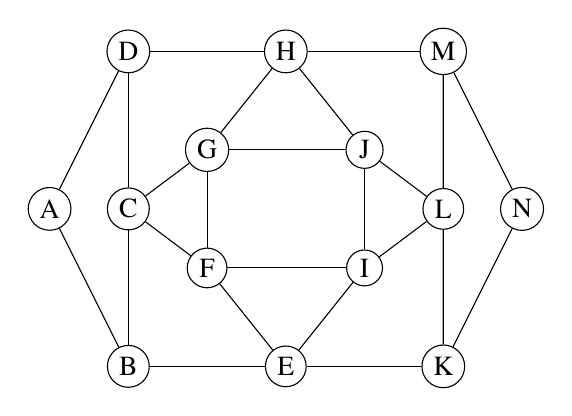
\begin{tikzpicture}[scale=1,
  every node/.style={circle, draw=black, fill=white, inner sep=2pt, minimum size=6pt},
  every edge/.style={draw=black, thick}
]

\node (A)  at (0, 2)    {A};  % was T
\node (B)  at (1, 0)    {B};  % was L2
\node (C)  at (1, 2)    {C};  % was C2
\node (D)  at (1, 4)    {D};  % was R2
\node (E)  at (3, 0)    {E};  % was L3
\node (F)  at (2, 1.25) {F};  % was CL3
\node (G)  at (2, 2.75) {G};  % was CR3
\node (H)  at (3, 4)    {H};  % was R3
\node (I)  at (4, 1.25) {I};  % was IML
\node (J)  at (4, 2.75) {J};  % was IMR
\node (K)  at (5, 0)    {K};  % was L6
\node (L)  at (5, 2)    {L};  % was C6
\node (M)  at (5, 4)    {M};  % was R6
\node (N)  at (6, 2)    {N};  % was B

% ---- Edges (same connectivity as original) ----
\draw (A) -- (B);
\draw (A) -- (D);
\draw (B) -- (C) -- (D);
\draw (N) -- (K) -- (L) -- (M) -- (N);
\draw (B) -- (E) -- (K);
\draw (E) -- (I) -- (L) -- (J) -- (H) -- (G) -- (C) -- (F) -- (E);
\draw (D) -- (H) -- (M);
\draw (F) -- (G) -- (J) -- (I) -- (F);
\end{tikzpicture}
\end{minipage}

\vfill

\begin{minipage}{0.45\textwidth}{
\vspace*{-1.3in} 
(b) (5 pts.) \emph{Duplicate} the \emph{fewest} number of edges such that the resulting graph will have an Euler circuit.  Note: You do not have to find the circuit.}
\end{minipage}
\hfill
\begin{minipage}{0.45\textwidth}
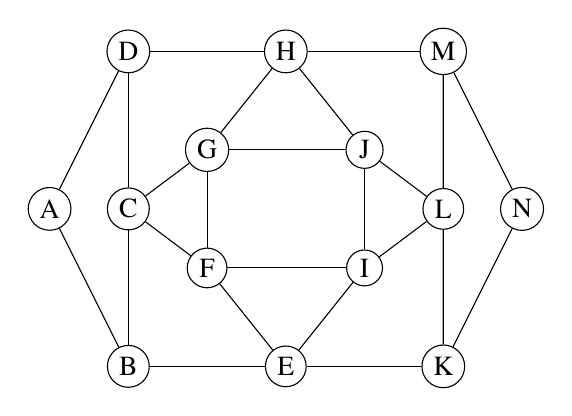
\begin{tikzpicture}[scale=1,
  every node/.style={circle, draw=black, fill=white, inner sep=2pt, minimum size=6pt},
  every edge/.style={draw=black, thick}
]

\node (A)  at (0, 2)    {A};  % was T
\node (B)  at (1, 0)    {B};  % was L2
\node (C)  at (1, 2)    {C};  % was C2
\node (D)  at (1, 4)    {D};  % was R2
\node (E)  at (3, 0)    {E};  % was L3
\node (F)  at (2, 1.25) {F};  % was CL3
\node (G)  at (2, 2.75) {G};  % was CR3
\node (H)  at (3, 4)    {H};  % was R3
\node (I)  at (4, 1.25) {I};  % was IML
\node (J)  at (4, 2.75) {J};  % was IMR
\node (K)  at (5, 0)    {K};  % was L6
\node (L)  at (5, 2)    {L};  % was C6
\node (M)  at (5, 4)    {M};  % was R6
\node (N)  at (6, 2)    {N};  % was B

% ---- Edges (same connectivity as original) ----
\draw (A) -- (B);
\draw (A) -- (D);
\draw (B) -- (C) -- (D);
\draw (N) -- (K) -- (L) -- (M) -- (N);
\draw (B) -- (E) -- (K);
\draw (E) -- (I) -- (L) -- (J) -- (H) -- (G) -- (C) -- (F) -- (E);
\draw (D) -- (H) -- (M);
\draw (F) -- (G) -- (J) -- (I) -- (F);
\end{tikzpicture}
\end{minipage}


\vfill
%\begin{minipage}{0.45\textwidth}	
(c)  (4 pts.) Suppose the edges are now weighted (see below). {Duplicate} edges such that the resulting graph will have an Euler circuit of \textbf{smallest possible total weight.} Note: You do not have to find the circuit.\\

\vspace{.5 in}
%\end{minipage}	
%\hfill
%\begin{minipage}{0.45\textwidth}	
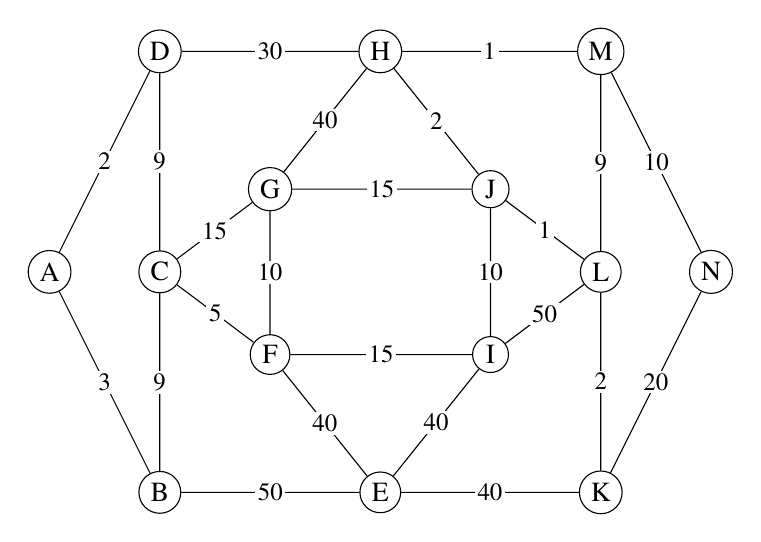
\begin{tikzpicture}[scale=1.4,
  every node/.style={circle, draw=black, fill=white, inner sep=2pt, minimum size=6pt},
  every edge/.style={draw=black, line width=1pt},
  rotate=90
]

% Node coordinates WITH LABELS
\node (T)  at (0, 6)   {A};

\node (L2) at (-2, 5) {B};
\node (C2) at (0, 5)  {C};
\node (R2) at (2, 5)  {D};

\node (L3) at (-2, 3)  {E};
\node (CL3) at (-0.75, 4) {F};
\node (CR3) at (0.75, 4)  {G};
\node (R3) at (2, 3)   {H};

\node (IML) at (-0.75, 2) {I};
\node (IMR) at (0.75, 2)  {J};

\node (L6) at (-2, 1) {K};
\node (C6) at (0, 1)  {L};
\node (R6) at (2, 1)  {M};

\node (B)  at (0, 0)  {N};

% Edge label style
\tikzset{
  wlabel/.style={
    rectangle, draw=none, fill=white,
    font=\small, inner sep=1pt
  }
}

% ---- Edges ----
\draw (T) -- node[wlabel]{3} (L2);
\draw (T) -- node[wlabel]{2} (R2);

\draw (L2) -- node[wlabel]{9} (C2) -- node[wlabel]{9} (R2);
\draw (CL3) -- node[wlabel]{10} (CR3);
\draw (IML) -- node[wlabel]{10} (IMR);
\draw (L6) -- node[wlabel]{2} (C6) -- node[wlabel]{9} (R6);

\draw (B) -- node[wlabel]{20} (L6);
\draw (R6) -- node[wlabel]{10} (B);

\draw (L2) -- node[wlabel]{50} (L3) -- node[wlabel]{40} (L6);
\draw (R2) -- node[wlabel]{30} (R3) -- node[wlabel]{1} (R6);

\draw (L3)  -- node[wlabel]{40} (IML) -- node[wlabel]{50} (C6);
\draw (C6)  -- node[wlabel]{1} (IMR) -- node[wlabel]{2} (R3);
\draw (CR3) -- node[wlabel]{15} (C2)  -- node[wlabel]{5} (CL3);
\draw (CL3) -- node[wlabel]{40} (L3);
\draw (CR3) -- node[wlabel]{40} (R3);
\draw (CR3) -- node[wlabel]{15} (IMR);
\draw (IML) -- node[wlabel]{15} (CL3);

\end{tikzpicture}
%\end{minipage}
	
\newpage
%%%%%%%%
%% Euler 2 
%%%%%%%%
\item (12 pts. total) There is a river running through the middle of a city with three islands and nine bridges, shown in the figure below.  

\vspace*{-.05in}
\begin{center}
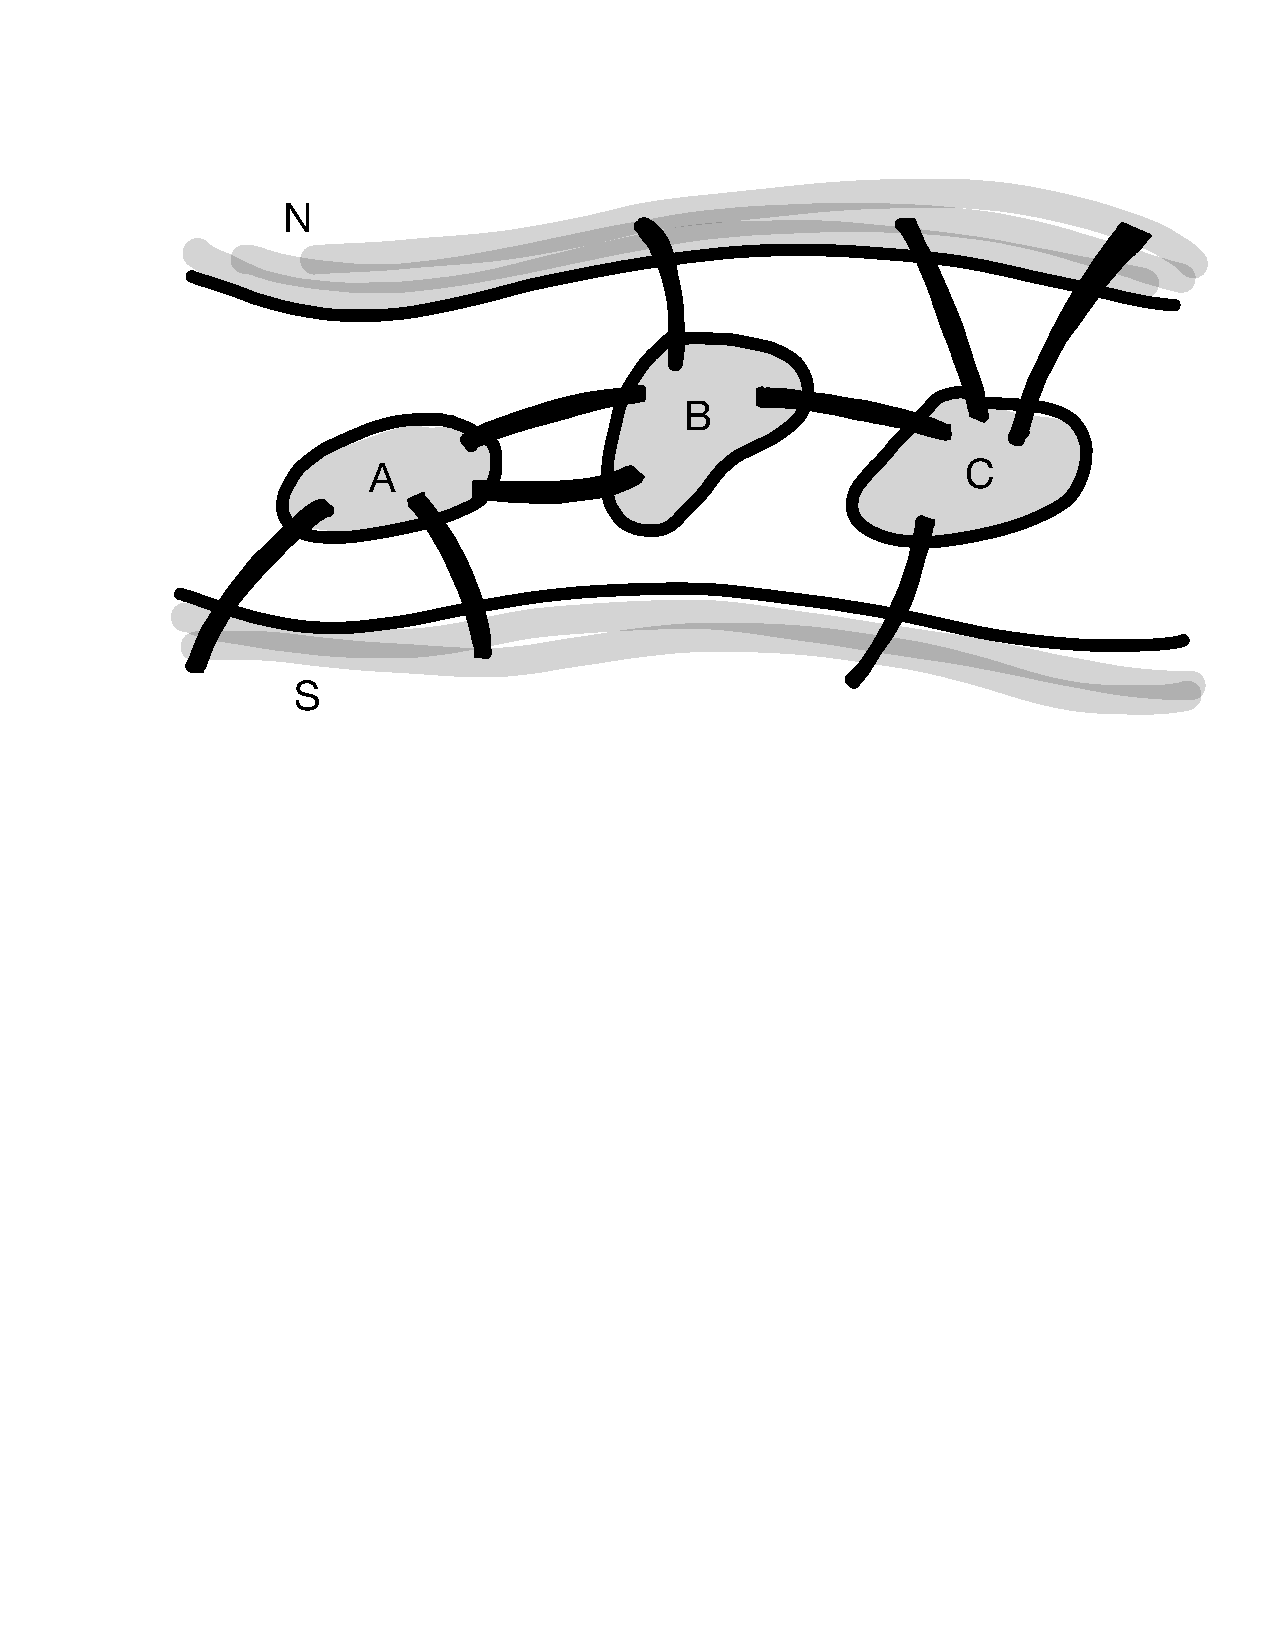
\includegraphics[scale=0.5]{Pic2.pdf}
\end{center}

	\begin{enumerate}
	\item (6 pts.) Draw a graph below that models this scenario. 
	
	\vfill
	\item (6 pts.) A tourist wants to travel from the South Bank ($S$) to the North Bank ($N$) going across every bridge \emph{at least} one time. Suppose there is a cost of \$2.00 every time one crosses a bridge. What is the cheapest \emph{achievable} cost of such a trip? Justify your answer.\\
	
	\textbf{cost:} \underline{\hspace{2in}}\\
	
	\textbf{justification:} \\
	
	\vfill
	\end{enumerate}
\newpage
%%%%%%%%%%%%%%
%%% Hamiltonian Circuit Question 1
%%%%%%%%%%%%%%
\item (12 pts.~total) A company plans to run a bus continually throughout the day in a loop around 5 tourist stops in a city, denoted A, B, C, D, and E. The company would like to find a route that minimizes the time to complete a loop. Driving times in minutes are shown in the table.

\begin{center}
\begin{tabular}{|c||c|c|c|c|c|}
\multicolumn{6}{c}{Driving Times in Minutes}\\
\hline
& {A} & {B} & {C} & {D} & {E} \\
\hline\hline
{A} & - & 4 & 7 & 3 & 2 \\
\hline
{B} & 4 & - & 5 & 6 & 9 \\
\hline
{C} & 7 & 5 & - & 8 & 6 \\
\hline
{D} & 3 & 6 & 8 & - & 5 \\
\hline
{E} & 2 & 9 & 6 & 5 & - \\
\hline
\end{tabular}
\end{center}

\begin{enumerate}
\item (3 pts.) \textbf{Using terminology from Graph Theory}, what is the company looking for?
\vskip 1.in
\item (6 pts.)
Use the Sorted Edges / Cheapest Link algorithm to find a good route for the bus. A table of driving times in increasing order is given. You may draw your route connecting the vertices provided if you wish, but be sure to also give your answer as a list of vertices, along with the total time on the bus.
\vspace{0.5cm}
\begin{center}
\begin{minipage}{2.in}
\begin{tikzpicture}[
    vertex/.style={circle, draw=black, inner sep=2pt, minimum size=6mm}
]
    \def\n{5}
    \def\radius{2cm}
     \def\angleDiff{72}
      \foreach \i/\label in {0/A, 1/B, 2/C, 3/D, 4/E} {
        \node[vertex] (v\label) at ({\i * \angleDiff}:\radius) {$\label$};
    }
    \end{tikzpicture}
    \end{minipage}
\hspace{1.cm}
\begin{minipage}{2.in}
\begin{tabular}{|c|c|c|}
\hline
edge& time &used?\\
\hline\hline
AE& 2&\\
\hline
AD&3&\\
\hline
AB&4&\\
\hline
BC&5&\\
\hline
DE&5&\\
\hline
CE&6&\\
\hline
BD&6&\\
\hline
AC&7&\\
\hline
CD&8&\\
\hline
BE&9&\\
\hline
\end{tabular}
\end{minipage}
 \end{center}
 
 
 \ 
   
   Route (list vertices)  \underline{\hskip2.in}
   
   \ 
   
   Total time on bus  \underline{\hskip2.in} 
   
   \ 
   
\item (3 pts.)  What other algorithm might you use for this problem if you were not confident that you had found the best route?

\
\end{enumerate}
\newpage
%%%%%%%%%
%% Longest Path
%%%%%%%%%
\item (12 pts. total) Answer the following questions about the graph drawn below. A copy of the vertices are provided to use as scratch work if desired. 

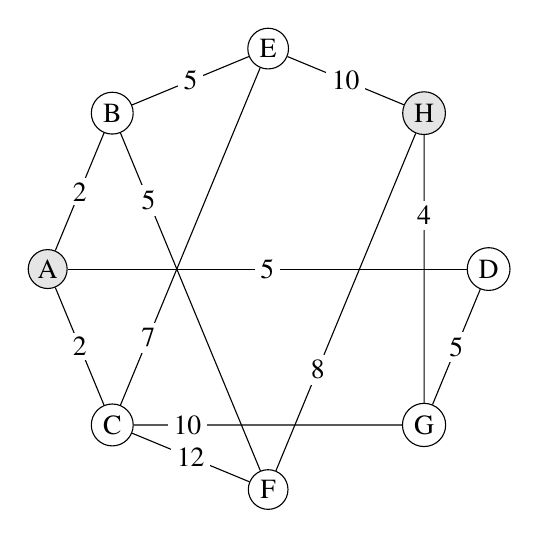
\begin{tikzpicture}[scale=1.4]
\node[draw,circle, inner sep=1.5pt, fill = gray!20](a) at (180:2){A};
\node[draw,circle, inner sep=2pt](b) at (180-45:2){B};
\node[draw,circle, inner sep=2pt](c) at (180+45:2){C};
\node[draw,circle, inner sep=2pt](d) at (0:2){D};
\node[draw,circle, inner sep=2pt](e) at (90:2){E};
\node[draw,circle, inner sep=2pt](f) at (270:2){F};
\node[draw,circle, inner sep=2pt](g) at (-45:2){G};
\node[draw,circle, inner sep=2pt,fill = gray!20](h) at (45:2){H};
\draw (a) -- (b) node [midway,inner sep=1.5pt,fill = white]{2};
\draw (a) -- (c) node [midway,inner sep=1.5pt,fill = white]{2};
\draw (a) -- (d) node [midway, inner sep = 2pt, fill = white]{5};
\draw (b) -- (f) node [pos = .2, inner sep = 2pt, fill = white]{5};
\draw (b) -- (e) node [midway,inner sep = 2pt, fill = white]{5};
\draw (c) -- (e) node [pos = .2,inner sep = 2pt, fill = white]{7};
\draw (c) -- (f) node [midway,inner sep = 2pt, fill = white]{12};
\draw (c) -- (g) node [pos = .2,inner sep = 2pt, fill = white]{10};
\draw (e) -- (h) node [midway,inner sep = 2pt, fill = white]{10};
\draw (h) -- (f) node [pos = .7,inner sep = 2pt, fill = white]{8};
\draw (h) -- (g) node [pos = .3,inner sep = 2pt, fill = white]{4};
\draw (g) -- (d) node [midway,inner sep = 2pt, fill = white]{5};
\end{tikzpicture}
\hspace{1in}
\begin{tikzpicture}[scale=1.4]
\node[draw,circle, inner sep=1.5pt, fill = gray!20](a) at (180:2){A};
\node[draw,circle, inner sep=2pt](b) at (180-45:2){B};
\node[draw,circle, inner sep=2pt](c) at (180+45:2){C};
\node[draw,circle, inner sep=2pt](d) at (0:2){D};
\node[draw,circle, inner sep=2pt](e) at (90:2){E};
\node[draw,circle, inner sep=2pt](f) at (270:2){F};
\node[draw,circle, inner sep=2pt](g) at (-45:2){G};
\node[draw,circle, inner sep=2pt,fill = gray!20](h) at (45:2){H};
\end{tikzpicture}
\vfill
\begin{enumerate}
\item (4 pts.) Find a shortest path from vertex A to vertex H. State the vertices on the path and its total weight. You are not required to use any particular method. \\

shortest path: \underline{\hspace{2in}} \hspace{0.5in} total weight: \underline{\hspace{2in}}\\

\vfill
\item (8 pts.) Describe one real-world situation for which finding a shortest path would be useful.\\

	\begin{enumerate}
	\item The vertices represent \hrulefill \\
	\vfill

	\item There is an edge between two vertices if \hrulefill\\
	\vfill

	\item The weight of edge represents \hrulefill\\
	\vfill

	\item Reason to find a shortest path:
	
	

\vspace{2in}
	\end{enumerate}
\end{enumerate}
\newpage
%%%%%%%%
%% Dijkstra's
%%%%%%%%
\item (10 pts. total) In this question you will be asked to do \emph{only a few steps} Dijkstra's Algorithm. We will suppose the goal of applying Dijkstra's Algorithm is to find a shortest path from $A$ to $G$ but \emph{at no point are you asked to complete Dijkstra's Algorithm from beginning to end or to actually find the shortest path.}\\
\begin{center}
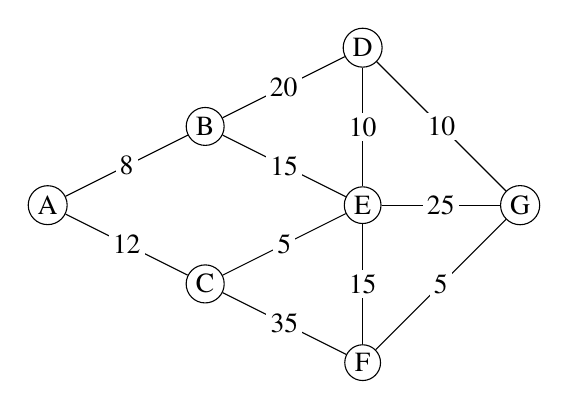
\begin{tikzpicture}
\node[draw,circle, inner sep=1.5pt](A) at (0,0){A};
\node[draw,circle, inner sep=1.5pt](B) at (2,1){B};
\node[draw,circle, inner sep=1.5pt](C) at (2,-1){C};
\node[draw,circle, inner sep=1.5pt](D) at (4,2){D};
\node[draw,circle, inner sep=1.5pt](E) at (4,0){E};
\node[draw,circle, inner sep=1.5pt](F) at (4,-2){F};
\node[draw,circle, inner sep=1.5pt](G) at (6,0){G};
\draw (A) -- (B) node [midway,inner sep=1.5pt,fill = white]{8};
\draw (A) -- (C) node [midway,inner sep=1.5pt,fill = white]{12};
\draw (B) -- (D) node [midway,inner sep=1.5pt,fill = white]{20};
\draw (B) -- (E) node [midway,inner sep=1.5pt,fill = white]{15};
\draw (C) -- (E) node [midway,inner sep=1.5pt,fill = white]{5};
\draw (C) -- (F) node [midway,inner sep=1.5pt,fill = white]{35};
\draw (D) -- (E) node [midway,inner sep=1.5pt,fill = white]{10};
\draw (E) -- (F) node [midway,inner sep=1.5pt,fill = white]{15};
\draw (D) -- (G) node [midway,inner sep=1.5pt,fill = white]{10};
\draw (E) -- (G) node [midway,inner sep=1.5pt,fill = white]{25};
\draw (F) -- (G) node [midway,inner sep=1.5pt,fill = white]{5};
\end{tikzpicture}
\end{center}
\begin{enumerate}
\item (5 pts.) Begin Dijkstra's Algorithm as though you seek a shortest path from $A$ to $G$, showing your work in the table below. \emph{STOP} when you mark a \emph{second} vertex as current.\\ DO NOT GO PAST THIS POINT. DO NOT DO THE WHOLE ALGORITHM.\\

\begin{tabular}{ |c | c |c| c|}
 \hline
 &&\textbf{tentative}&\\
 vertex & current/ & minimum& preceding\\ 
 &visited&\quad distance to $G$ \quad& vertex\\
 \hline
A&&& \\
\hline 
B&&& \\
\hline 
C&&& \\
\hline 
D&&& \\
\hline 
E&&& \\
\hline 
F&&& \\
\hline
G&&& \\
\hline
 \end{tabular}
\vfill

\item (5 pts.) A few more steps of Dijkstra's Algorithm have been completed for you. Identify the \emph{next current vertex} and update the appropriate rows in the table below. \emph{STOP} once your current vertex is marked as \emph{visited}.
\vfill
\begin{minipage}{0.5\textwidth}
  \centering
\begin{tabular}{ |c | c |c| c|}
 \hline
 &&\textbf{tentative}&\\
 vertex & current/ & minimum& preceding\\ 
 &visited&\quad distance to $G$ \quad& vertex\\
 \hline
A&&& \\
\hline 
B&&30& D\\
\hline 
C&&40&F \\
\hline 
D&\cancel{C}, V&10&G \\
\hline 
E&&\cancel{25} 20&\cancel{G} F\\
\hline 
F&\cancel{C}, V&5&G \\
\hline
G&\cancel{C}, V&0& $-$\\
\hline
 \end{tabular}
\end{minipage}%
\begin{minipage}{0.5\textwidth}
 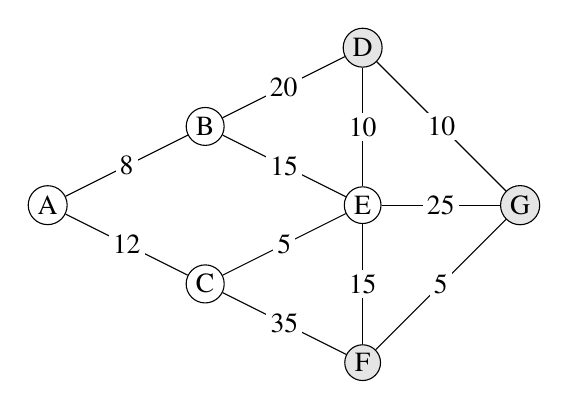
\begin{tikzpicture}
\node[draw,circle, inner sep=1.5pt](A) at (0,0){A};
\node[draw,circle, inner sep=1.5pt](B) at (2,1){B};
\node[draw,circle, inner sep=1.5pt](C) at (2,-1){C};
\node[draw,circle, inner sep=1.5pt, fill =gray!20](D) at (4,2){D};
\node[draw,circle, inner sep=1.5pt](E) at (4,0){E};
\node[draw,circle, inner sep=1.5pt, fill =gray!20](F) at (4,-2){F};
\node[draw,circle, inner sep=1.5pt, fill =gray!20](G) at (6,0){G};
\draw (A) -- (B) node [midway,inner sep=1.5pt,fill = white]{8};
\draw (A) -- (C) node [midway,inner sep=1.5pt,fill = white]{12};
\draw (B) -- (D) node [midway,inner sep=1.5pt,fill = white]{20};
\draw (B) -- (E) node [midway,inner sep=1.5pt,fill = white]{15};
\draw (C) -- (E) node [midway,inner sep=1.5pt,fill = white]{5};
\draw (C) -- (F) node [midway,inner sep=1.5pt,fill = white]{35};
\draw (D) -- (E) node [midway,inner sep=1.5pt,fill = white]{10};
\draw (E) -- (F) node [midway,inner sep=1.5pt,fill = white]{15};
\draw (D) -- (G) node [midway,inner sep=1.5pt,fill = white]{10};
\draw (E) -- (G) node [midway,inner sep=1.5pt,fill = white]{25};
\draw (F) -- (G) node [midway,inner sep=1.5pt,fill = white]{5};
\end{tikzpicture}
\end{minipage}

\end{enumerate}

\newpage
%%%%%%%%%%
%%% SET UP Scheduling
%%%%%%%%%
\item (15 pts total) Consider the following table of tasks and
dependencies.

\begin{tabular}{c | c | c}
Task & Time & dependency\\
\hline
A & 3 hours & \\
B & 4 hours & \\
C & 6 hours & \\
D & 8 hours & A,B\\
E & 5 hours & B \\
F & 1 hour & C\\
G & 2 hours & D,E,F \\
\end{tabular}

\begin{enumerate}
\item (5 pts.) Construct a {\bf scheduling digraph} corresponding to the
  tasks and dependencies above.\\
  
  \vfill
\item (2 pts.) What priority list do you get if you prioritize the tasks using
the {\bf Decreasing Time Algorithm}?\\

\vspace{1in}
\item (5 pts.) Apply the {\bf
    Backflow Algorithm} to find the critical time for each task. \emph{Use square brackets} -- [ ] -- for these labels.\\
    
    
\item (3 pts.) What priority list do you get if you prioritize the tasks using
  the {\bf Critical Path Algorithm}?\\
  \vspace{1in}
\end{enumerate}

\newpage

%%%%%%%%%%%%%%
%%% Make a Schedule
%%%%%%%%%%%%%%

%%%% Graph for Next Problem
\def\r{1}
\def\s{.9}
\newcommand{\anotherdigraph}{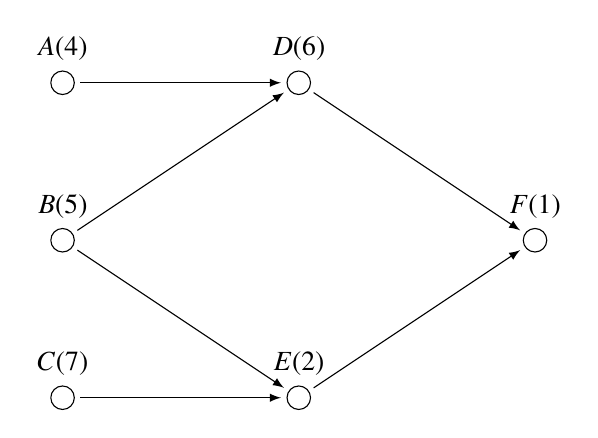
\begin{tikzpicture}[vtx/.style={draw, circle, inner sep = 3pt, %font = \scriptsize
}, myto/.style={-latex, shorten >=2pt, shorten <=2pt
}, node distance = \r cm]

\node[vtx, label=above:{$A(4)$}, ] (A) at (0,4){};
\node[vtx, label=above:{$B(5)$}, ] (B) at (0,2){};
\node[vtx, label=above:{$C(7)$}, ] (C) at (0,0){};
\node[vtx, label=above:{$D(6)$}, ] (D) at (3,4){};
\node[vtx, label=above:{$E(2)$}, ] (E) at (3,0){};
\node[vtx, label=above:{$F(1)$}, ] (F) at (6,2){};
\foreach \i/\j in {A/D,B/D,B/E,C/E,D/F,E/F}{\draw[myto] (\i) -- (\j);}
\end{tikzpicture}
}

\item (15 pts) Consider the following digraph. The units for the tasks are \emph{hours}.
\begin{center}
\anotherdigraph 
\end{center}
\vfill
\begin{enumerate}

\item (10 pts) Construct a schedule for two processors using the \emph{priority list }
\[ E,\;\;A,\;\;D,\;\;F,\;\;C,\;\;B\]

Make sure to label the tasks in the schedule. You may use the table below to track your work.


\vfill
\hspace*{-1cm}	\begin{tabular}{c || c}
time &   \quad \hspace{6in} \quad \\ \hline
done& \\ \hline
ready& \\ \hline
\end{tabular}
\vfill
%\vspace{-1cm}
%\begin{center}
\hspace{-1cm}
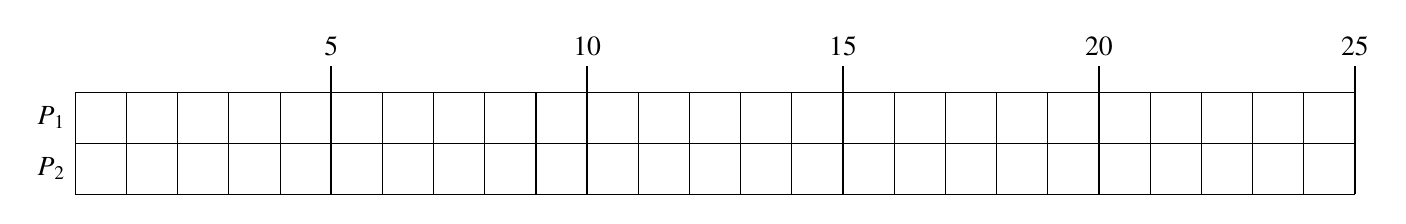
\begin{tikzpicture}[scale = 1.3, lbl/.style={font=\tiny, inner sep = 1 pt, fill = white}]
\path (0, 3/4) node[left] {$P_{1}$};
\path (0, 1/4) node[left] {$P_{2}$};
\draw[step=1/2] (0,0) grid (25/2, 2/2);
\foreach \i in {5, 10, ..., 25}{\draw[thick] (\i/2,0) -- (\i/2,2/2+1/4) node[ above]{\i};}
\end{tikzpicture} 
%\end{center}

\vfill

\item (3 pts) How much \emph{idle time} is in this schedule?%, and when?
 \hrulefill
\vfill
\item (2 pts.) How long did this schedule take to complete? \ans
\vfill
\end{enumerate}

\newpage
%%%%%%%%%%
%%Extra Credit
%%%%%%%%%%
Extra Credit (4 pts.) Below is the floor plan of an art gallery with 6 galleries and 11 doorways.  A security company has assigned a theft risk assessment for each doorway. The higher the number the greater the risk. 

\vspace{.3in}

%%%%% OLD
\begin{center} 
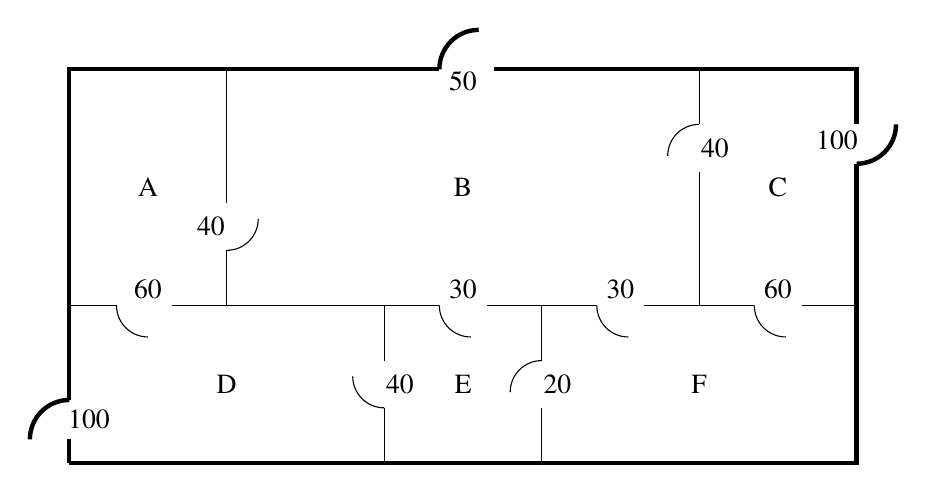
\begin{tikzpicture}
%% outside
\draw[ultra thick] (0,0)--(0,5) -- (10,5) -- (10,0) -- (0,0);
%% inside walls
\draw (0,2) -- (10,2);
\draw (2,2) -- (2,5)(4,0)--(4,2)(6,0)--(6,2)(8,2) -- (8,5);
%%% bust holes in walls
\draw[ultra thick, white] (4.7,5) -- (5.4,5)(10, 3.8 ) -- (10, 4.3 )(0,0.3)--(0,0.8);
\draw[ultra thick, white] (0.6,2) -- (1.3,2)(4,0.7)--(4,1.3)(6,0.7)--(6,1.3);
\draw[ultra thick, white] (4.7 ,2) -- (5.3 , 2)(6.7 ,2) -- (7.3 , 2)(8.7 ,2) -- (9.3 , 2);
\draw[ultra thick, white] (2,2.7 )-- (2,3.3)(8,3.7)--(8,4.3);
\node at (0.25,0.55){100};
\node at (1,2.2){60};
\node at (4.2,1){40};
\node at (6.2,1){20};
\node at (5,2.2){30};
\node at (7,2.2){30};
\node at (9,2.2){60};
\node at (1.8,3){40};
\node at (8.2,4){40};
\node at (5,4.85){50};
\node at (9.75,4.1){100};
\node at (1,3.5){A};
\node at (5,3.5){B};
\node at (9,3.5){C};
\node at (2,1){D};
\node at (5,1){E};
\node at (8,1){F};
%%% Door arcs

% B to outside (top wall)
\draw[ultra thick] (5,5) ++(-0.3,0) arc (180:90:0.5);
% C to outside (right)
\draw[ultra thick] (10,4.1) ++(0,-0.3) arc (-90:0:0.5);
% D to outside (left wall)
\draw[ultra thick]  (0,.3) ++(-0.5,0) arc (180:90:0.5);
% BE door
\draw (4.7,2) arc (180:270:0.4);
% CF door
\draw (8.7,2) arc (180:270:0.4);
% BF door
\draw (6.7,2) arc (180:270:0.4);
% AD door
\draw (.6,2) arc (180:270:0.4);
% D-E door
\draw (4,1.1) ++(-0.4,0) arc (180:270:0.4);
% E-F door
\draw (6,1.3) arc (90:180:0.4);
% BC door
\draw (8,4.3) arc (90:180:0.4);
% AB door
\draw (2,2.7) arc (270:360:0.4);
\end{tikzpicture}
\end{center}

\begin{enumerate} 
\item Draw a graph below that models this scenario.
\vfill

\item The gallery owners want all rooms to be available to visitors but they would like to shut and lock as many doors as possible to lower their risk.  \textbf{Using terminology from Graph Theory},  what is the company looking for?
\vfill
\end{enumerate}


% ---- Interior doors ----

%% A-B door
%\draw (4.7,2) arc (180:270:0.3);
%
%% B-C door
%\draw (5.3,2) arc (0:-90:0.3);
%
%% A-D door
%\draw (2,3.7) arc (90:0:0.3);
%
%% B-E door
%\draw (4,1.3) arc (90:0:0.3);
%
%% B-E second connection (top-bottom)
%\draw (6,1.3) arc (90:180:0.3);
%
%% C-F door
%\draw (8,3.7) arc (90:180:0.3);
%
%% D-E door
%\draw (4,0.7) arc (180:90:0.3);
%
%% E-F door
%\draw (6,0.7) arc (0:90:0.3);
%
%\end{tikzpicture}




\end{enumerate}
\end{document}

